
\section{Results}

\begin{figure}
\centering
\begin{tabular}{cc}
\subfloat {
\includegraphics[width=4cm]{images/original_2}} & 
\subfloat {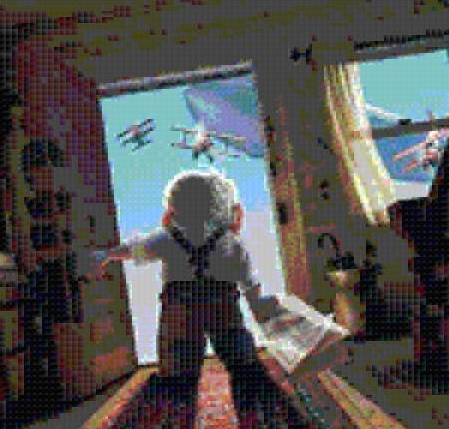
\includegraphics[width=4cm]{images/reconstructed_2}} & 
\end{tabular}
\caption{Visual comparison of original and reconstructed image.}
\label{fig:compare_images}
\end{figure}


We tested the compression algorithm with 100 images which were not in the training set and get a mean error of 0.0086 and a compression rate of 0.0094. 
We also tested with 100 images which were all in the training set and the mean error was 0.0082 and the compression rate 0.0092. 
%Time for everything: 907.7797 \newline
%Average quadratic error: 0.0086154 \newline
%Average compression rate: 0.0094089 \newline
%Average inverse for sum compression/error 55.4806 \newline


\newline
%and with 100 images which are all in the training set:\newline
%Time for everything: 873.8136 \newline
%Average quadratic error: 0.008281 \newline
%Average compression rate: 0.0092095 \newline
%Average inverse for sum compression/error 57.174
%\newline
Figure~\ref{fig:compare_images} shows an example image before any compression on the left and the reconstructed image after compression on the right. 
\newline
As in (TODO: Reference to paper) we also tried to do the training directly on the actual image only. The results were worse than the pre-training. The compression rate was the same, but the mean error was 0.173.  
%Time for everything: 44.1702
%Average quadratic error: 0.17375
%Average compression rate: 0.0086164
%Average inverse for sum compression/error 5.4836



\newline
TODO: Run program with different parameters and construct graphs to compare results.

\subsection{Comparison to Baselines}
We compare our solution with two baselines. The first baseline is a compression algorithm based on Principal Component Anlaysis(PCA) and the second algorithm is based on Clustering with Gaussian Mixture Models(GMM).  
\newline
In PCA, one projects high dimensional data to low dimensional data. This can be done using the eigenvalue decomposition on the covariance matrix $\Sigma$, which describes the covariance matrix as a product of three matrices U, $\Lambda$ and U$^T$. U contains the eigenvectors of  $\Sigma$ and $\Lambda$ contains the eigenvalues of $\Sigma$. Similar to SVD, one can sort the eigenvalues in decreasing order and then take the k largest of them and the first k columns of U and k columns of U$^T$ to reduce the data which has to be saved. 
\newline
\newline
TODO: Mention parameters used for both baselines, e.g k
\newline
\newline
Clustering is the process of assigning each value x in a data set S to some value x' of a smaller set S'. In image compression one can use this to reduce the color space. Each pixel is assigned to one of the RGB values in the smaller color set, i.e. to a cluster. Using mixture models, each pixel can be assigned to more than one cluster with a corresponding probability. In a gaussian mixture model, those values are distributed according to a normal distribution. The second baseline compresses images with this approach. 
\newline
TODO:
\newline
Compare compression rates.... 
\newline
Compare error....
